% !TEX encoding = UTF-8
% !TEX TS-program = pdflatex
% !TEX root = ../tesi.tex

%**************************************************************
\chapter{Analisi dei Requisiti}
\label{cap:processi-metodologie}
%**************************************************************
Durante il primo periodo di tirocinio è stata svolta la fase di Analisi dei Requisiti, necessaria alla comprensione del dominio e al soddisfacimento della richiesta. Inizialmente è stato effettuato un incontro con il tutor aziendale con il quale sono stati rilevati i requisti obbligatori richiesti dall'azienda da cui è stato possibile identificare un insieme di funzionalità necessarie alla Skill. Successivamente è stato realizzato il documento contenente tutti gli studi di analisi che hanno favorito una buona e corretta progettazione del prodotto. Dalla raccolta dei dati e dalle analisi fatte è stata elaborata una visione ad alto livello del sistema e dei rispettivi casi d’uso. Sono stati inoltre identificati quei punti critici in grado di determinare, in larga misura, la forma finale del prodotto.
La fase di analisi si è infine conclusa con lo studio della VUI (Voice User Interface), e della GUI (Graphical User Interface), che caratterizzano l'esperienza d'uso del prodotto finale. 

%**************************************************************
\section{Obbiettivo}
L’obiettivo del progetto di stage è la realizzazione di una Skill per l’assistente vocale Alexa che sia in grado di accogliere clienti, postini e corrieri all'ingresso degli uffici e notificare in maniera automatica la persona interessata nell'arrivo del visitatore. La Skill è concepita per essere installata sui dispositivi in commercio da Amazon, in particolare sul dispositivo Echo Show 2018. L’obiettivo è quindi quello di realizzare un concierge virtuale che accolga il visitatore e riceva da esso informazioni per mezzo di una conversazione e l’uso di messaggi attraverso lo schermo touch integrato nel dispositivo. In fine tali dati elaborati dai processi di controllo per inviare notifiche al personale.

\subsection{Cliente finale}
Il cliente finale a cui è destinato il prodotto è l’azienda Crispy Bacon Srl, la quale necessita, per ovvi motivi, di un sistema automatizzato che svolga il ruolo di Concierge all'entrata degli uffici. L’azienda desidera, con questo prodotto, realizzare uno prototipo da poter rendere spendibile tale servizio proponendolo come pacchetto preconfezionato o da personalizzare al fine di venderlo a clienti terzi.

\section{Attori coinvolti}
Dall'analisi fatta sono emersi i seguenti attori, intesi come persone coinvolte nell'utilizzo della Skill:
\begin{itemize}
    \item Visitatore
        \begin{itemize}
            \item Persona avente appuntamento
            \item Persona non avente appuntamento
            \item Postino
            \item Corriere
        \end{itemize}
    \item Personale di Crispy Bacon
\end{itemize}

\section{Requisiti richiesti}
I requisiti emersi e richiesti dall'azienda sono stati elaborati e analizzati. Tali requisiti sono interpretabili in tre diversi modi, tutti sotto il presupposto che questi siano in qualche modo una necessità.
\begin{itemize}
    \item Requisito utente: dal punto di vista dell'utente, è una capacità necessaria per risolvere un problema o raggiungere un obbiettivo.
    \item Requisito software: dal punto di vista della soluzione, è una capacità che deve essere posseduta dal sistema per adempiere all'obiettivo.
    \item Dal punto di vista della documentazione, come una descrizione documentata di una capacità interpretata come un requisito utente o software.
\end{itemize}
\subsubsection{Identificazione dei Requisiti}
Per identificare i requisti viene utilizzata la seguente notazione tabellare con un codice che lo identifica e la corrispettiva descrizione affianco.
\begin{center}
    R.x.y
\end{center}
\begin{itemize}
    \item R: identifica il requisito
    \item x: identifica l'importanza di tale requisito che può essere
        \begin{itemize}
            \item O obbligatorio
            \item D desiderabile
        \end{itemize}
    \item y: identifica un valore numerico progressivo a partire da 1
\end{itemize}
In merito allo studio di analisi fatto all'inizio del periodo di tirocinio sono emersi i seguenti requisti, \textbf{considerati obbligatori} per il soddisfacimento del risultato atteso dal prodotto finale.
\begin{center}
	\centering
	\renewcommand{\arraystretch}{1.5}
	\rowcolors{3}{tableLight}{}
	\begin{longtable}{  p{2.5cm} p{9.8cm} }
		\rowcolor{tableHead}
		\textbf{\textcolor{white}{Identificativo}} & \textbf{\textcolor{white}{Requisito}} \\
		\endhead  
		RO1 & La Skill al momento dal lancio deve presentare un messaggio di benvenuto (\textbf{VUI}) \\
		RO2 & La Skill al momento dal lancio deve presentare un messaggio di benvenuto (\textbf{GUI}) \\
		RO3 & La Skill al momento dal lancio deve presentare un elenco essenziale e sintetico delle azioni da fare (\textbf{VUI}) \\ 
		RO4 & La Skill al momento dal lancio deve presentare un elenco essenziale e sintetico delle azioni da fare  (\textbf{GUI}) \\
		RO5 & La Skill deve poter ricevere le informazioni necessarie dal visitatore per mezzo di una conversazione impostata (\textbf{VUI})  \\
		RO6 & La Skill deve poter riportare le informazioni ottenute dal visitatore e riportarle nello schermo del dispositivo (\textbf{GUI}) \\
		RO7\label{RO7} & La Skill deve poter utilizzare e interrogare il servizio di calendarizzazione con le informazioni ottenute dal visitatore al fine di notificare l'interessato della visita.\\
		RO8\label{RO8} & La Skill deve notificare o inviare una notifica all'interessato della visita.\\
		RO9 & La Skill deve riportare sullo schermo del dispositivo delle funzioni disponibili in base alle risposte ricevute dal dialogo fatto con il visitatore (\textbf{GUI - VUI})\\
		\rowcolor{white}
		\caption{Tabella tracciamento requisiti obbligatori}
	\end{longtable}
\end{center}
Infine nell'analisi sono stati individuati anche i \textbf{requisiti desiderabili}, considerati non strettamente necessari ma di valore aggiunto al prodotto atteso.
\begin{center}
	\centering
	\renewcommand{\arraystretch}{1.5}
	\rowcolors{3}{tableLight}{}
	\begin{longtable}{  p{2.5cm} p{9.8cm} }
		\rowcolor{tableHead}
		\textbf{\textcolor{white}{Identificativo}} & \textbf{\textcolor{white}{Requisito}} \\
		\endhead  
		RD1 & La Skill una volta verificata la presenza del visitatore informa quest'ultimo se l'interessato risulta non reperibile se assente \\
		RD2 & La Skill deve poter registrare il momento in cui il visitatore inizia l'incontro con la persona cercata nel caso di un appuntamento \\
		RD3 & La Skill deve poter registrare il momento in cui il visitatore termina l'incontro con la persona cercata nel caso di un appuntamento \\
		\rowcolor{white}
		\caption{Tabella tracciamento requisiti desiderabili}
	\end{longtable}
\end{center}
\section{Casi d'uso}
Dalle analisi fatte e dai dati raccolti sono stati studiati i requisiti funzionali, ovvero i casi d'uso del prodotto Concierge Crocante, che permettono di descrivere interazioni tra gli utenti, tra il sistema e come quest'ultimo deve essere utilizzato. Durante lo stage sono stati così esaminate le sequenze di passi che descrivono interazioni e la rappresentazione di possibilità, che hanno in comune uno scopo finale per un utente (attore).\\[0.4cm]
Gli attori emersi nell'analisi dei casi d’uso svolgono il ruolo dell'utente nell'interazione con la Skill per raggiungere l’obiettivo prefissato. In questa analisi sono stati individuati gli attori:
    \begin{itemize}
        \item Utente generico, che può essere generalizzato in:
            \begin{itemize}
                \item Visitatore
                    \begin{itemize}
                        \item avente appuntamento
                        \item non avente appuntamento
                        \item postino
                        \item corriere
                    \end{itemize}
                \item Persona cercata
        \end{itemize}
    \end{itemize}
Di seguito viene riportato lo schema degli attori individuati utilizzando lo standard UML 2.0
\begin{figure}[H] 
    \centering 
    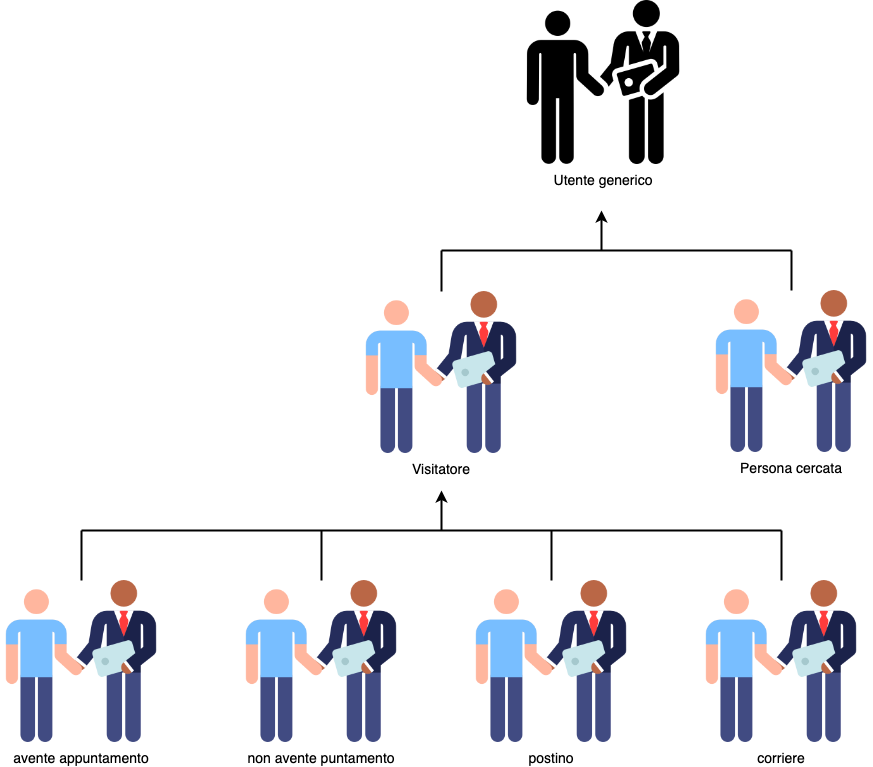
\includegraphics[width=0.9\columnwidth]{immagini/attori.png}
    \caption{\label{fig:attori}Utenti del sistema}
\end{figure}
\subsection{Casi d'uso - Persona}
\subsection{Casi d'uso - Postino/Corriere}
